\documentclass[a4paper,12pt]{article}
\usepackage{amsmath}
\usepackage{amssymb}
\usepackage{tikz}
\usepackage{tkz-euclide}
\usepackage{hyperref}
\usetikzlibrary{shapes.geometric, calc, decorations.markings}
\usepackage{geometry}
\usepackage{footnote}
\usepackage{setspace}
\usepackage{fancyhdr}

\geometry{a4paper, total={170mm,257mm}, left=20mm, right=20mm, top=20mm, bottom=20mm}

\title{Tetrahedron with Six Pentagons Geometry and the Lynchpin Concept of Terrence Howard}
\author{Marko T. Manninen}
\date{\today}

\begin{document}

\maketitle

\begin{abstract}
\noindent
This study investigates the geometric angle discrepancy in a tetrahedron compared to a pentagon within the framework of Terrence Howard's Lynchpin concept. Although the numerical value of this geometric discrepancy resembles the Pythagorean comma in music theory, our analysis demonstrates that they are from different mathematical basis. We offer practical methods to measure and demonstrate this discrepancy in both musical terms (cents) and physical terms (millimeters). An interactive 3-D model is provided to further investigate and visualize the Lynchpin concept.
\end{abstract}

\section*{Keywords}
Tetrahedron, Pentagon, Geometric discrepancy, Lynchpin concept, Terrence Howard, Eric Weinstein, Pythagorean comma, Solid angles, Centroid, 3-D model, Geometric analysis, Musical intervals, Engineering applications, Joe Rogan Experience

\thispagestyle{empty}

\onehalfspacing

\pagestyle{fancy}
\fancyhf{}
\fancyhead[C]{\thepage}


\section{Background}
In the conversation between American mathematician Eric Weinstein and actor Terrence Howard on the Joe Rogan Experience (JRE) \#2171 (beginning at 2:49:08 and ending at 3:01:25), they discuss Howard's concept of the Lynchpin and its geometric and other implications.

The term lynchpin commonly refers to something or someone essential to an organization, system, or situation, holding all the various elements together whose failure or removal could lead to the collapse or dysfunction of a larger structure. Originally, a lynchpin was a physical pin passed through the end of an axle to keep a wheel in place, crucial for the functioning of wheeled vehicles.

Howard explains his Lynchpin as a fundamental element or lowest common denominator of all matter, involving concepts like the internal dimensions of a torus and universal wave conjugation.

Weinstein critiques theories that claim to explain everything with a single principle, such as string theory, which posits that particles are vibrating strings. He expresses concern whether such "mass delusions" could also be associated with the Lynchpin concept.

While the details of the Lynchpin implications are not well elaborated in the interview, we have enough hints to review the Lynchpin geometry. Implications are discussed in the wider context in Howard's OTOET eBook, pages 124 and 145. (\href{https://tcotlc.com/wp-content/uploads/2020/09/OTOET_PREVIEW_055_SEPTEMBER_29_2020.pdf}{PDF})

Weinstein suggests that Howard's Lynchpin discovery might be based on a mathematical error but acknowledges its beauty and potential. When Howard references the Pythagorean comma as a discrepancy in this regard, Weinstein states, "Now we are talking about it!" Weinstein draws an analogy between the Pythagorean comma—a small frequency interval that illustrates imperfections in musical tuning systems—and the geometrical issues in Howard's Lynchpin concept.

Weinstein proposes that, despite the flaw, Howard's Lynchpin concept might have engineering potential due to its ability to give six geometrical degrees of freedom in design. A small, unavoidable discrepancy, similar in scale to the Pythagorean comma, might fall within engineering error margins and tolerances.

Weinstein's use of the words "error" and "flaw" should not be interpreted as implying that Howard has overlooked the discrepancy or that there is a fault in the mathematical calculations of the Lynchpin. However, it is not clear from the discussion whether Terrence has directly related the geometric angle discrepancy to the Pythagorean comma. In this document, we demonstrate that these discrepancies originate from different bases and are not evidently related even if their values are approximately the same.

Moreover, Weinstein did not acknowledge that Howard has already demonstrated a practical patented application by conducting a competition in 2021. Three participants built drone devices based on the Lynchpin concept showing successful engineering proof, which Howard awarded with a prize. (\href{https://www.terryslynchpins.com/welcome-to-now}{Website})

Earlier in the JRE \#2127 discussion (01:13:40), Weinstein highlighted several instances where fundamental geometric structures, analogous to Platonic solids, have yielded practical applications. Notable examples include the Rubik's cube, introduced in 1974, and Hoberman's Switch-Pitch ball, developed in 2001.

Finally, Weinstein referenced viral capsids (03:08:58)—protein shells that exhibit nearly perfect icosahedral symmetry—as functional biological entities. These examples challenge the notion that foundational geometric concepts from antiquity lack contemporary relevance or that biological forms rely exclusively on ideal geometries.

For the full conversation, refer to Joe Rogan Experience \#2171 - Eric Weinstein \& Terrence Howard on July 1, 2024. (\href{https://www.youtube.com/watch?v=nrOaFxNex7U}{YouTube})


\section{Tetrahedron Basics}
A tetrahedron is a three-dimensional polyhedron with four triangular faces, six straight edges, and four vertices. The tetrahedron is one of the simplest and most symmetric platonic solids.

\begin{center}
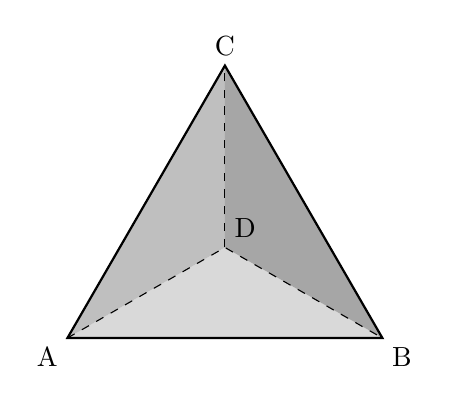
\begin{tikzpicture}
    \coordinate (A) at (0,0);
    \coordinate (B) at (4,0);
    \coordinate (C) at (2,3.46);
    \coordinate (D) at (2,1.15);

    % Draw and shade the faces
    \fill[gray!30] (A) -- (B) -- (D) -- cycle;
    \fill[gray!50] (A) -- (D) -- (C) -- cycle;
    \fill[gray!70] (B) -- (D) -- (C) -- cycle;

    % Draw the edges
    \draw[thick] (A) -- (B) -- (C) -- cycle;
    \draw[dashed] (A) -- (D) -- (B);
    \draw[dashed] (D) -- (C);

    % Label the vertices
    \node[below left] at (A) {A};
    \node[below right] at (B) {B};
    \node[above] at (C) {C};
    \node[above right] at (D) {D};
\end{tikzpicture}
\end{center}

\noindent
The above diagram shows a tetrahedron with vertices \( A \), \( B \), \( C \), and \( D \). Each edge is of equal length, and each face is an equilateral triangle. Each internal angle of the equilateral triangles that form the faces is \( 60^\circ \).


\section{Centroid of the Tetrahedron}
The centroid of a tetrahedron is the point where the four medians intersect. It is the center of mass of the tetrahedron and is located at an equal distance from all four vertices. This can also be seens as the radius of the circumscribed sphere, which passes through all four vertices and is centered at the centroid, and is considered to be of unit length (1) in the following example.

The centroid can be found by averaging the coordinates of the vertices. If the vertices of the tetrahedron are given as \( A(x_1, y_1, z_1) \), \( B(x_2, y_2, z_2) \), \( C(x_3, y_3, z_3) \), and \( D(x_4, y_4, z_4) \), then the coordinates of the centroid \( G \) are given by:

\[
G \left( \frac{x_1 + x_2 + x_3 + x_4}{4}, \frac{y_1 + y_2 + y_3 + y_4}{4}, \frac{z_1 + z_2 + z_3 + z_4}{4} \right)
\]

\begin{center}
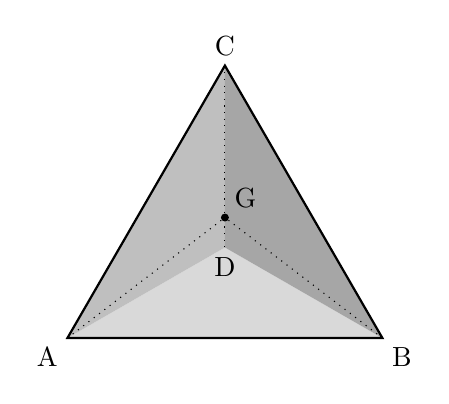
\begin{tikzpicture}
    \coordinate (A) at (0,0);
    \coordinate (B) at (4,0);
    \coordinate (C) at (2,3.46);
    \coordinate (D) at (2,1.15);
    \coordinate (G) at (2,1.53);

    % Draw and shade the faces
    \fill[gray!30] (A) -- (B) -- (D) -- cycle;
    \fill[gray!50] (A) -- (D) -- (C) -- cycle;
    \fill[gray!70] (B) -- (D) -- (C) -- cycle;
    
    \draw[thick, fill=black] (2,1.53) circle(1pt);

    % Draw the edges
    \draw[thick] (A) -- (B) -- (C) -- cycle;
    \draw[transparent] (A) -- (D) -- (B);
    \draw[transparent] (D) -- (C);

    % Draw the dashed lines
    \draw[dotted] (A) -- (G);
    \draw[dotted] (B) -- (G);
    \draw[dotted] (C) -- (G);
    \draw[dotted] (D) -- (G);

    % Label the vertices
    \node[below left] at (A) {A};
    \node[below right] at (B) {B};
    \node[above] at (C) {C};
    \node[below] at (D) {D};
    \node[above right] at (G) {G};
\end{tikzpicture}
\end{center}

\noindent
The diagram shows the tetrahedron with its centroid \( G \). The dotted lines represent the four medians connecting the vertices to the centroid.


\section{Internal Angle from the Centroid to the Vertices}
The internal angle from the centroid \( G \) of the tetrahedron to its vertices \( A \), \( B \), \( C \), and \( D \) can be calculated as follows:

1. \textbf{Vector Calculation}: Consider vectors from the centroid \( G \) to any of the vertices, for example, \( \overrightarrow{GA} \), \( \overrightarrow{GB} \), etc.

2. \textbf{Dot Product}: The dot product of any two vectors from the centroid to two vertices is:
   \[
   \overrightarrow{GA} \cdot \overrightarrow{GB} = |GA| \cdot |GB| \cdot \cos(\theta)
   \]
   Since the vectors are of equal length (since \( G \) is equidistant from all vertices), and given that the tetrahedron is regular, the dot product simplifies using the edge length and the centroid coordinates.

3. \textbf{Derivation of the Angle}: For a regular tetrahedron, this dot product calculation leads to:
   \[
   \cos(\theta) = -\frac{1}{3}
   \]
   Therefore, the angle \(\theta\) is:
   \[
   \theta = \arccos\left(-\frac{1}{3}\right) \approx 109.47^\circ
   \]

\noindent
This angle is sometimes referred to simply as the tetrahedral angle. There are totally six such angles formed inside the tetrahedron, each to be matched with two regular pentagon sides in the Lynchpin.


\section{Pentagon Geometry}
Next, let's explore the geometric properties of a regular pentagon, where the side length is equal to the radius of the circumscribed sphere of the tetrahedron, which is considered to be of unit length.

A regular pentagon is a five-sided polygon with equal side lengths and equal internal angles.

\begin{center}
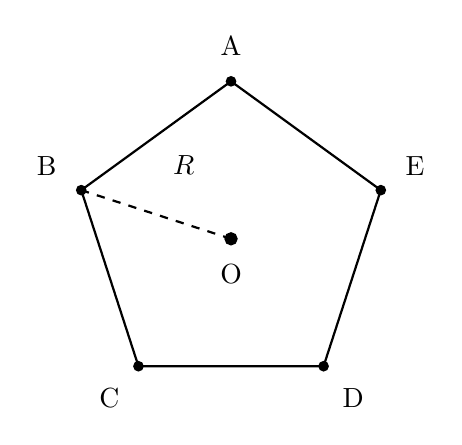
\begin{tikzpicture}
    \draw[thick] (18:2) -- (90:2) -- (162:2) -- (234:2) -- (306:2) -- cycle;
    \foreach \x in {18, 90, 162, 234, 306}
        \draw[thick, fill=black] (\x:2) circle(1.5pt);

    \draw[thick, fill=black] (0,0) circle(2pt);
    \draw[dashed, thick] (0,0) -- (162:2);

    \node[above] at (90:2.2) {A};
    \node[above left] at (162:2.2) {B};
    \node[below left] at (234:2.2) {C};
    \node[below right] at (306:2.2) {D};
    \node[above right] at (18:2.2) {E};
    \node[below] at (0,-0.2) {O};
    \node[left] at (-250:1) {$R$};
\end{tikzpicture}
\end{center}

\noindent
Each internal angle of a regular pentagon is:
\[
\alpha = \frac{(5-2) \times 180^\circ}{5} = 108^\circ
\]

\noindent
To find the radius of the circumscribed circle around the pentagon, we use the relationship between the side length \( s \) of the pentagon and the radius \( R \):

\[
s = 2R \sin\left(\frac{\pi}{5}\right) \approx 1.176 \cdot R
\]

\noindent
Given that \( s = 1 \) and solving for \( R \):

\[
R = \frac{1}{2 \sin\left(\frac{\pi}{5}\right)} \approx 0.85
\]

\noindent
Thus, the radius of the circumscribed circle \( R \) around the pentagon with a side length of 1 is approximately 0.85 units. This radius is useful to draw pentagon vertices for the interactive 3-D model of the Lynchpin.

To produce the Lynchpin geometry, the task is to match tetrahedron side GA and GB with pentagon side AB and AE, respectively, and do it for all six internal tetrahedron angles: AGB, AGC, AGD, BGC, BGD, and CGD. (See also Figure \ref{fig:3d-lynchpin})

\begin{figure}[h]
\centering
\includegraphics[width=\textwidth]{3d-lynchpin.png}
\caption{3-D representation of the Lynchpin geometry, where six pentagon vertices meet at the centroid of the tetrahedron. For an interactive 3-D model, visit the \href{https://markomanninen.github.io/lynchpin}{Lynchpin GitHub-project webpage}.}
\label{fig:3d-lynchpin}
\end{figure}


\section{Tetrahedron and Pentagon Angle Discrepancy}
Comparing the internal angle from the centroid to the vertices in the tetrahedron (\( 109.47^\circ \)) with the internal angle of the pentagon (\( 108^\circ \)), we find a small discrepancy:
\[
109.47^\circ - 108^\circ = 1.47^\circ
\]

\noindent
The ratio of these angles is:
\[
\frac{109.47}{108} \approx 1.01361
\]

\noindent
See Figure \ref{fig:3d-lynchpin-error} for the visual representation of the discrepancy.

\begin{figure}[h]
\centering
\includegraphics[width=\textwidth]{3d-lynchpin-error.png}
\caption{3-D representation of the Lynchpin "error," where tetrahedron inner triangle sides (eg. 1 and 2) connect, while the respective pentagon sides (red and green) do not.}
\label{fig:3d-lynchpin-error}
\end{figure}


\section{Pythagorean Comma}
The Pythagorean comma is the small interval by which twelve perfect fifths (each with a frequency ratio of \( \frac{3}{2} \)) exceed seven octaves (each with a frequency ratio of 2). Mathematically, this is expressed as:
\[
\left(\frac{3}{2}\right)^{12} \approx 129.74634 \quad \text{and} \quad 2^7 = 128
\]
\[
\text{Pythagorean comma} = \frac{129.74634}{128} \approx 1.01364
\]


\section{Comparing the Ratios}
The ratio of the angle discrepancy in the geometric context (using \(\theta = \arccos(-\frac{1}{3})\)) is compared to the ratio of the Pythagorean comma. Using six-digit precision, the ratios are normalized to the same numerator and denominator for accurate comparison.

\subsection{Pythagorean Comma}

The Pythagorean comma ratio comes from prime numbers 2 and 3 and is expanded as follows:

\[
\left(\frac{3}{2}\right)^{12} \quad \text{to} \quad 2^7 = \frac{531441}{524288}
\]

\subsection{Geometric Ratio}

The tetrahedron internal angle to the internal angle of the pentagon is:
\[
\frac{109.4712206}{108} \approx \frac{109471}{108000}
\]

1. \textbf{Normalized Denominator}: Prime factorization by using a fixed Pythagorean comma numerator (531441):
\[
531441 = 3^{12}, \quad 524299 = 43 \times 89 \times 137
\]
Ratio:
\[
\frac{531441}{524299} \approx 1.013622
\]

2. \textbf{Normalized Numerator}: Prime factorization by using a fixed Pythagorean comma denominator (524288):
\[
531430 = 2 \times 5 \times 19 \times 2797, \quad 524288 = 2^{19}
\]
Ratio:
\[
\frac{531430}{524288} \approx 1.013615
\]

\subsection{Conversion to Cents}

In musical terms, a cent is a logarithmic unit of measure used for musical intervals. One cent is \( \frac{1}{100} \) of a semitone in the equal-tempered scale, where an octave is divided into 1200 equal parts. The formula to convert a ratio \( r \) to cents is:
\[
\text{Cents} = 1200 \times \log_2(r)
\]

\noindent
Applying this to the Lynchpin geometric discrepancy ratio:
\[
\text{Cents} = 1200 \times \log_2(1.01362) \approx 23.41 \, \text{cents}
\]

\noindent
Applying this to the Pythagorean comma ratio:
\[
\text{Cents} = 1200 \times \log_2(1.01364) \approx 23.45 \, \text{cents}
\]


\subsection{Real-life Comparison of the Discrepancy}

The smallest hearable difference in pitch, or a just noticeable difference (JND), is typically around 5 cents. The geometric angle discrepancy of approximately 1.47 degrees, corresponding to about 23.41 cents, is more than four times the JND. This means that the difference, though small, is perceptible to the human ear.

Also, when creating the Lynchpin with pentagons the size of a hand, the discrepancy becomes visible but not totally unmanageable. When the discrepancy angle between two sides of a 5 cm isosceles triangle (one of the side being pentagon's, other being tetrahedron radius) is 1.147122 degrees, the base length is approximately 1 mm (calculated using the simplified Law of Cosines: \( c^2 = 2a^2 (1 - \cos(\theta)) \), where \( a = 5 \) cm and \( \theta = 0.020019 \) degrees in radians).

It was demonstrated in Howard's competition, that three prize-awarded participants successfully created drone devices based on the Lynchpin geometry despite of this 1 mm scale discrepancy. (\href{https://www.terryslynchpins.com/welcome-to-now}{Website})


\section{Conclusion}
The Pythagorean comma and the geometric ratio demonstrate different principles: cyclic, multiplicative processes rooted in harmonic relationships and logarithmic scaling versus direct trigonometric measurements and spatial projections. Despite their similar numerical values for the first four decimals, the methods of achieving these ratios are distinct in their unique contexts. This is further examplified with the prime factorization discrepancy. Thus, we can only speak of analogous discrepancies between Pythagorean comma and the Lynchpin angles.

The Pythagorean comma necessitates temperaments in musical tuning to balance the discrepancies. Similarly, the geometric ratio discrepancy demands precise adjustments in engineering and design to maintain structural integrity. It might result challenges in mass-producing Lynchpin-inspired gadgets on ensuring functionality and reliability at scale.


\section{References}

\begin{thebibliography}{9}

\bibitem{joe-rogan}
Joe Rogan Experience \#2171 - Eric Weinstein \& Terrence Howard. July 1, 2024. Available at \url{https://www.youtube.com/watch?v=nrOaFxNex7U}.

\bibitem{lynchpin-competition}
Howard, Terrence. (2021). \emph{Terrence Howards Lynchpin drone competition}. Available at \url{https://www.terryslynchpins.com/welcome-to-now}.

\bibitem{ebook}
Howard, Terrence. (2020). \emph{One Times One Equals Two eBook, section about Lynchpin, pages 124, 145}. Available at \url{https://tcotlc.com/wp-content/uploads/2020/09/OTOET_PREVIEW_055_SEPTEMBER_29_2020.pdf}.

\bibitem{3d-model}
Manninen, Marko. (2024). \emph{Interactive 3-D model of the Lynchpin geometry at GitHub-project}. Available at \url{https://github.com/markomanninen/lynchpin}.

\end{thebibliography}

\end{document}